The final step of our method is to annotate the detected events in a human-readable way. We aim to generate short summaries so that the user does not have to process a large quantity of text, and can just skim through a few sentences to decide whether he is interested in that particular event. If so, then he can examine the event more closely and go through the actual documents, which we have retrieved in chapter \autoref{chap:document-retrieval}.

Although the keyword set discovered in \autoref{chap:event-detection} provides a concise representation of an event, it can lead to ambiguities or simply not reveal enough information. The keywords should be considered an internal representation used in the detection process, not something presentable to the user.


\begin{figure}[H]
  \centering
  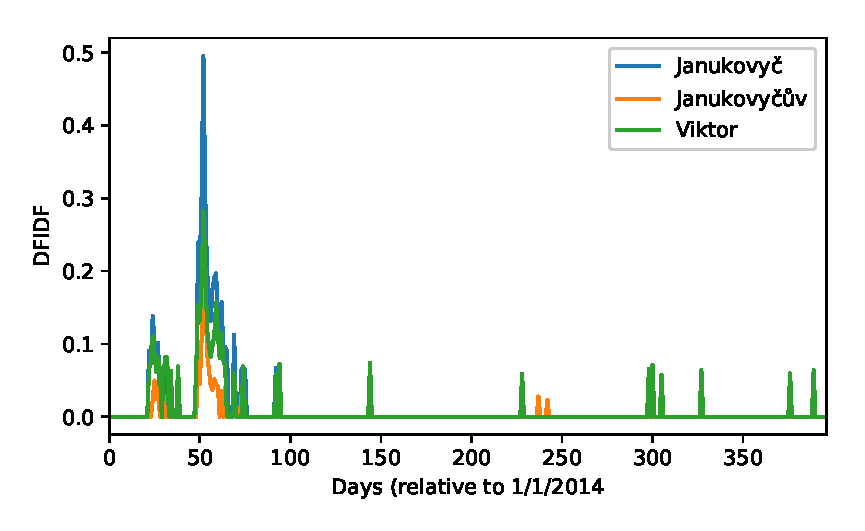
\includegraphics{18_words}  % original event
  \caption{An event concerning Viktor Yanukovych being ousted from Ukraine's presidency, which is not recognizable from the keyword set.}
  \label{fig:not-recognizable}
\end{figure}


A simple method is to annotate an event by the headline of the most relevant document in terms of Word Mover's Similarity. This may give insight of the general topic of the particular event, but it is unlikely that a whole event will be well characterized by a single document. For this reason, we also investigate a more complex method.

To obtain richer annotations, we apply multi-document summarization techniques to generate a short summary of an event's document set. More specifically, we attempt to extract a subset of sentences out of the event documents, which cover the general topic of the event without providing redundant information. As the documents come from different sources and describe the events from different perspectives, the result will not generally be a continuous paragraph, but more of a set of characteristic sentences. Still, a longer piece of text will likely provide a better insight into an event than a single headline.

We use the multi-document summarization system presented in \cite{multi-summarization-1, multi-summarization-2}, which we describe in more detail in the following paragraphs. This system was later improved by \cite{mogren-1}, who evaluated the usage of different word embedding techniques for sentence similarity measures. Their work led to the system presented in \cite{mogren-2} which aggregates several different similarity measures to obtain a better quality summary. We adapt such system and combine together several measures of sentence similarity suitable for the event detection task.


\section{Multi-document summarization}
In \cite{multi-summarization-1}, the authors formulate the task of multi-document summarization as a constrained combinatorial optimization problem, where the goal is to retrieve a subset of sentences maximizing a monotone submodular function $\quality{\cdot}$ measuring the summary quality.

A submodular function $\quality{\cdot}$ on a set of sentences $V$ satisfies the property of \textit{diminishing returns}; that is, for $A \subseteq B \subseteq V \setminus \{ v \},\ \quality{A \cup \{ v \}} - \quality{A} \geq \quality{B \cup \{ v \}} - \quality{B},\ v \in V$. This has an intuitive interpretation for text summarization, namely that adding a sentence $v$ to a longer summary does not improve the summary as much as adding it to a smaller one. The reason is that the information carried by $v$ is likely already present in the longer summary.

Even though solving the task exactly is NP-hard, a greedy algorithm is guaranteed to find a solution only a constant factor off the optimum, as discussed by the authors.

The summary quality is measured in terms of how representative it is to the whole set (coverage) and how dissimilar the sentences are to each other (diversity). The constraints limit the summary to a reasonable length by bounding either the number of sentences or the number of words.

In \cite{multi-summarization-1}, basic submodular functions to be used in multi-document summarization are described. In \cite{multi-summarization-2}, these functions are further developed to better capture the semantic properties of sentences.

Mathematically, the task is formulated as

\begin{equation}
\begin{alignedat}{-1}
\max_{S \subseteq V} & \quad \quality{S} = \coverage{S} + \lambda \diversity{S} \\
\text{s. t.} & \quad \sum_{i \in S}{\sentcost_{i}} \leq \budget,
\end{alignedat}
\end{equation}

where $V$ is the set of all sentences from the document set being summarized, $\sentcost_{i}$ is the cost of sentence $i$ (either 1 when limiting the number of sentences, or the number of words in the sentence otherwise) and $\budget$ is the total budget.

A feasible set $S$ maximizing $\quality{\cdot}$ will provide a reasonable number of sentences well capturing the overall topic of the whole document set, no two of which being redundant. What remains is to define the coverage function $\coverage{\cdot}$ and diversity function $\diversity{\cdot}$, whose influence can be controlled by the parameter $\lambda \geq 0$. Additionally, the functions must be defined in a way that the conditions from \cite{multi-summarization-1} are not broken, so that a greedy algorithm can still be used with performance guarantee.


\section{Coverage function}

In \cite{multi-summarization-2}, the coverage function $\coverage{\cdot}$ is defined in terms of pairwise sentence similarity $\semsim{\cdot}{\cdot}$ as

\begin{equation}
\coverage{S} = \sum_{i \in V}{\min{\Big\{ \sum_{j \in S}{\semsim{i}{j}}, \alpha \sum_{j \in V}{\semsim{i}{j}} \Big\} }}.
\end{equation}

The first argument of the minimum measures the similarity between the sentence $i$ and the summary $S$, while the second argument measures the similarity between the sentence $i$ and the rest of the sentences $V$. The number $\alpha \in [0,1]$ is a threshold coefficient controlling the influence of the overall similarity.

In \cite{multi-summarization-1}, the authors further prove that if $\semsim{i}{j} \in [0,1]\ \forall i, j \in V$, the whole function remains submodular.

Originally, only a simple cosine similarity between TFIDF sentence vectors \citep{information-retrieval} was used as $\semsim{\cdot}{\cdot}$. \cite{mogren-1} examined various methods of word embeddings to obtain a finer measure of similarity. This alone outperformed the original method. In \cite{mogren-2}, a more complex system aggregating multiple similarity measures was built, further improving the summary quality. The authors compute the sentence similarity $\semsim{i}{j}$ as a product of these individual similarities, all bounded in $[0, 1]$: $\semsim{i}{j} = \prod_{l}{\similarity_{s_{i}, s_{j}}^{l}}$.

We use this method with several different similarity measures fit for the event detection task. Next, we describe the individual sentence similarities used.

\subsection{TFIDF similarity}

The first measure used is the standard cosine similarity between TFIDF (Term Frequency-Inverse Document Frequency) vectors \citep{information-retrieval} of two sentences $s_{i}$ and $s_{j}$. Such method is a simple measure of document similarity often used in information retrieval.

If we denote the frequency of the word $w$ in sentence $s_{i}$ as $\text{tf}_{w,i}$ and the inverse document frequency of $w$ as $\text{idf}_{w}$, the similarity is written as

\begin{equation}
	\similarity_{s_{i}, s_{j}} = \frac{\sum_{w \in s_{i} \cup s_{j}} \text{tf}_{w,i} \cdot \text{tf}_{w,j} \cdot \text{idf}_{w}^{2}}{\sqrt{\sum_{w \in s_{i}} \text{tf}_{w, i}^{2} \cdot \text{idf}_{w}^{2}} \cdot \sqrt{\sum_{w \in s_{j}} \text{tf}_{w, j}^{2} \cdot \text{idf}_{w}^{2}}}.
\end{equation}

The term frequencies are always non-negative, and so the whole cosine similarity is in $[0, 1]$.

The major setback of TFIDF similarity is that it does not go beyond simple word overlap, though weighted to diminish stopwords and amplify important words. That means that if two sentences convey essentially the same information through different vocabulary, they will not be ranked similar due to having only a few words in common. That can be a problem in larger document collections from different sources and authors.

\subsection{Word2Vec similarity}

We attempt to solve this problem by considering the word embeddings of the individual words, as first examined by \cite{mogren-1}.

We represent a sentence $s_{i}$ by summing together the vector embeddings of its words, $\embed_{i} = \sum_{w \in s_{i}} \embed_{w}$. The similarity of two sentences is then the cosine similarity of these vectors, transformed to $[0, 1]$:

\begin{equation}
	\similarity_{s_{i}, s_{j}} = \left(\frac{\inp{\embed_{i}}{\embed_{j}}}{\| \embed_{i} \| \cdot \| \embed_{j} \|} + 1 \right) / \ 2.
\end{equation}

This similarity brings a finer distinction of word-level semantics. This means that even if two sources reporting the same event use fairly different vocabularies, the sentences will still be ranked similar.

\subsection{TR similarity}

The next measure uses Text Rank (TR) similarity, as defined by \cite{textrank}. Each sentence is represented by a set of words, and the overlap of these sets is measured. \cite{mogren-2} achieved best results by combining the TFIDF similarity, word embeddings and the TR similarity, which is defined as

\begin{equation}
	\similarity_{s_{i}, s_{j}} = \frac{\left| s_{i} \cap s_{j} \right|}{\log{\left| s_{i} \right|} + \log{\left| s_{j} \right|}}.
\end{equation}


\subsection{Keyword similarity}

In addition to the three previously described similarities, \cite{mogren-2} considered a keyword similarity, which measures the overlap between two sentences and a predefined keyword set. Having previously obtained the event keyword representation $\kw{e}$, we use this measure to make sure the sentences actually concern the particular event.

The similarity is defined as 

\begin{equation}
	\similarity_{s_{i}, s_{j}} = \frac{\sum_{w \in \left( s_{i} \cap s_{j} \cap \kw{e} \right)} \text{tf}_{w} \cdot \text{idf}_{w}}{\left| s_{i} \right| + \left| s_{j} \right|}.
\end{equation}

The measure effectively chooses only those sentences having non-zero word overlap with the keyword set. It also breaks the summary fluency, making the summary more of a set of sentences characteristic for the given event. On the other hand, the resulting sentences will be highly relevant to the event, often revealing important information about it.

This tradeoff between fluency and quality is more worth it when summarizing a large number of documents. Even without the keyword similarity, the chance that two summary sentences will make sense consecutively is quite small, when they come from different documents.

If an event consisted of only one or two documents, it would make sense to use a different measure to reach better fluency.

\section{Diversity function}

Now, we can define the diversity function, which will positively reward a summary consisting of non-redundant sentences. \cite{multi-summarization-2} again defined the function in terms of a simple TFIDF similarity. We only redefine the function to accept the custom similarity function built in the previous steps.

The diversity of a summary $S$ is based on clustering the sentences by their similarity $\semsim{\cdot}{\cdot}$ and then preferrably choosing sentences from different clusters not similar to each other. Formally, the function is defined as

\begin{equation}
	\diversity{S} = \sum_{k = 1}^{K} \sqrt{\sum_{j \in S \cap P_{k}} r_{j}},
\end{equation}

where $P_{k},\ k = 1, \dots, K$ is a clustering of the sentence set $V$. The value $r_{j} = \frac{1}{N} \sum_{i \in V} \semsim{i}{j}$ is the singleton reward for adding the sentence $i$ into the summary $S$.

This function positively rewards diverse sentences in a sense that once an element $i$ from a cluster $P_{k}$ is chosen, other elements from the same cluster will have diminishing gains due to the square root function (see \cite{multi-summarization-2} for a concrete example). This means that if the clustering partitions the sentences into semantically different clusters, the summary will draw from different semantical categories and will consist of sentences conveying different information.

We apply the K-Medoids algorithm with $\semsim{\cdot}{\cdot}$ as a custom distance function.


\section{Optimization}
Having defined the cost function $\quality{\cdot}$, we can use the greedy algorithm defined in \cite{multi-summarization-1} to obtain the desired summary.

For the experiments, we set a budget of 50 words. In the diversity function the number of clusters $K$ was set to $\frac{\left| V \right|}{10}$, putting 10 sentences into each cluster on average. As for the other parameters, we used the values from the original papers \citep{multi-summarization-1, multi-summarization-2}. The list of generated summaries can be found in \autoref{app:clusters-events}.